\section{Semaine 7 : 20/03/2023 - 24/03/2023}
\graphicspath{{semaines/semaine_7/images/}}

\begin{abstract}
	Lundi : Après discussion avec Michel des résultats obtenus les semaines précédentes, on a décidé de se concentrer sur la comparaison des erreurs PhiFEM, FNO et avec la correction (avec la méthode extrapolate de FEniCS). On a également parlé d'entrainer le modèle avec des données plus fines (nb\_vert=128). Sur ma machine, ça n'a pas été possible (OOM : Out Of Memory). Je me suis donc connectée à Titan sur lequel l'entrainement a également crashé (Noyau mort). Je pense que le problème vient de l'installation de tensorflow (car j'ai cloné sur Titan l'environnement conda phifem) : il faudrait tester d'installer htop pour voir si la RAM est pleine. C'est un problème qui est mis de côté pour l'instant.
	
	Mardi : Après discussion avec Michel et Emmanuel, Emmanuel a proposé de regarder les facteurs de division d'erreur sur la solution analytique pour différents $\mathbb{P}^k$. (Ensuite, on a une réunion d'équipe sur les FNO) Puis, une fois ces résultats obtenus, Michel a proposé de vérifier les pentes de convergence au niveau de l'interpolation de la level-set et sur la correction. Il a également proposé une nouvelle idée pour faire en sorte que la correction soit moins couteuse que PhiFEM classique : On entraine le réseau en $32\times 32 \; \mathbb{P}^2$ puis on applique la correction sur du $\mathbb{P}^1$ puis on compare les erreurs (PhiFEM, FNO et FNO+Corr).
	
	Pour le reste de la semaine, on s'est alors concentré sur cette nouvelle idée pour le FNO. La première complexité a été de pouvoir faire le passage d'une solution $\mathbb{P}^2$ de Numpy à FEniCS et de FEniCS à Numpy. Au vue des résultats obtenus sur la solution analytique trigonométrique, on pense qu'il est possible que les données soient "trop simple" (ne varie pas assez) pour que la correction ait un intérêt. En effet, il semblerait qu'un entrainement de seulement 500 époques nous donnent déjà de très bons résultats avec le FNO. La correction a alors du mal à corriger la solution obtenue par le FNO car elle est déjà très bonne. Pour justifier cette hypothèse, on choisit de changer le problème considéré : on repasse à Poisson avec condition de Dirichlet homogène où on prend $f$ gaussienne. Comme l'on a pas de solution analytique pour ce problème, on considérera une solution sur-raffinée comme solution de référence. 
\end{abstract} \; \\

On considérera dans la suite deux normes. La première norme est une norme relative calculée avec FEniCS :
$$||y_{true}-y_{pred}||^2_{L^2(\Omega_h),rel}=\frac{\int_{\Omega_h}(y_{true}-y_{pred})^2}{\int_{\Omega_h}y_{true}^2}$$
La seconde est calculée à partir des "images" représentées par des tableaux Numpy ou des tenseurs :
$$||y_{true}-y_{pred}||^2_2=\frac{1}{N^2}\sum_{i=1}^{N}\sum_{j=1}^{N} (y_{true}(i,j)-y_{pred}(i,j))^2*mask$$
où $N$ est nb\_vert.

(PS : j'aurais du mettre la seconde norme en norme relative.)

\subsection{Comparaison PhiFEM, FNO et FNO+Corr}

On considère la solution analytique trigonométrique suivante :
$$u_{ex}(x,y) = \frac{1}{\sin\left(k_1\frac{\pi}{2}\right)}\times\sin\left(k_1\frac{\pi}{2}\left(\frac{4}{\sqrt{2}}\right)^2\left((x-0.5)^2+(y-0.5)^2\right)\right)\times\cos\left(\frac{\pi}{2}\left(\frac{4}{\sqrt{2}}\right)^2\left((x-0.5)^2+(y-0.5)^2\right)\right)\,, $$ 

On entraîne notre FNO avec nb\_vert=64, nb\_data=1000 et sur 1000 époques. On calcule alors les normes relatives suivantes :
$$||u_{ex}-u_{PhiFEM}||_2, \; ||u_{ex}-u_{FNO}||_2, \; ||u_{ex}-u_{Corr}||_2$$
où la méthodes choisi pour la correction est une extrapolation de degré 2 et 3.

\newpage On obtient les résultats suivants :

\begin{minipage}{\linewidth}
	\centering
	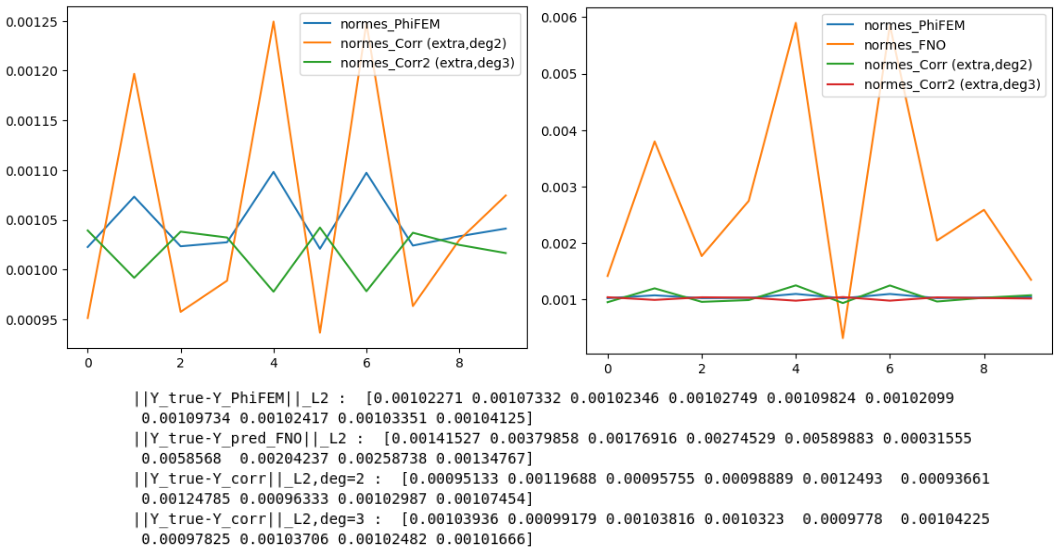
\includegraphics[width=0.9\linewidth]{comp_PhiFEM_FNO_Corr.png}
\end{minipage}

\subsection{Facteurs de division de l'erreur sur la solution analytique}

On considère encore la solution analytique trigonométrique suivante :
$$u_{ex}(x,y) = \frac{1}{\sin\left(k_1\frac{\pi}{2}\right)}\times\sin\left(k_1\frac{\pi}{2}\left(\frac{4}{\sqrt{2}}\right)^2\left((x-0.5)^2+(y-0.5)^2\right)\right)\times\cos\left(\frac{\pi}{2}\left(\frac{4}{\sqrt{2}}\right)^2\left((x-0.5)^2+(y-0.5)^2\right)\right)\,, $$ 

On cherche ici à déterminer les facteurs de division entre PhiFEM et la correction appliqué à la solution analytique. Voici les résultats obtenus :

\begin{minipage}{\linewidth}
	\centering
	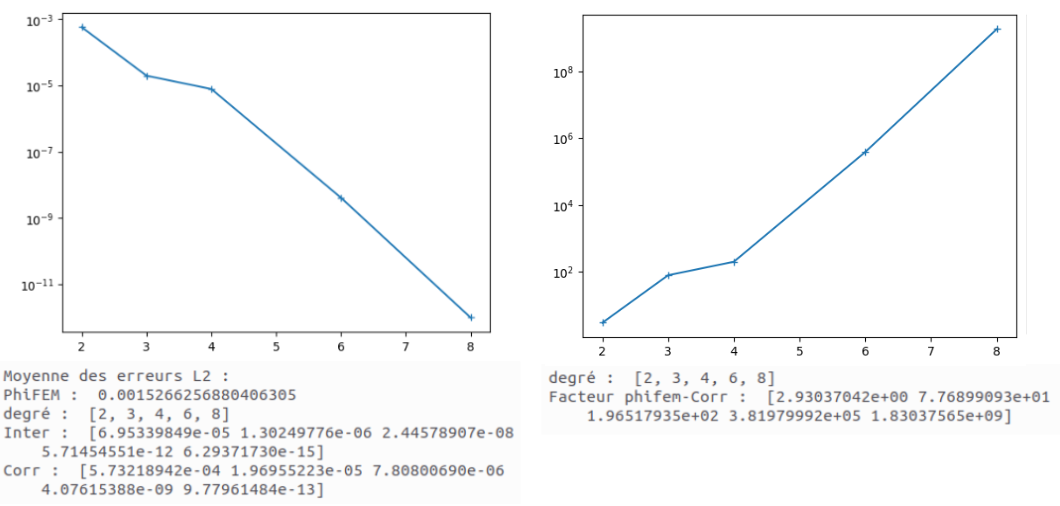
\includegraphics[width=0.8\linewidth]{test_degre.png}
\end{minipage}

\subsection{Pentes de convergence (interpolation et correction)}

On veut vérifier ici les pentes des droites de convergence sur la norme $L^2$ de la différence entre la solution exacte et son interpolation :
$$||u_{ex}-I_h u_{ex}||_{L^2(\Omega_h),rel}\sim h^{k+1}$$
Dans un second temps on cherche à déterminer numériquement la pente des droites de convergence sur la norme $L^2$ de la différence entre la solution exacte et la correction appliquée à son interpolation :
$$||u_{ex}-CI_h u_{ex}||_{L^2(\Omega_h),rel}\sim h^{?}$$

On traitera dans un premier temps le cas avec la solution analytique trigonométrique puis le cas où f est gaussienne où on prend comme solution de référence une solution sur-raffinée.

\subsubsection*{Solution analytique trigonométrique}

On considère encore la solution analytique trigonométrique suivante :
$$u_{ex}(x,y) = \frac{1}{\sin\left(k_1\frac{\pi}{2}\right)}\times\sin\left(k_1\frac{\pi}{2}\left(\frac{4}{\sqrt{2}}\right)^2\left((x-0.5)^2+(y-0.5)^2\right)\right)\times\cos\left(\frac{\pi}{2}\left(\frac{4}{\sqrt{2}}\right)^2\left((x-0.5)^2+(y-0.5)^2\right)\right)\,, $$ 

On considère la solution exacte $u_{ex}$ interpolé à un ordre assez élevé (de degré 8 par exemple). On interpole cette solution exacte (notre nouvelle level-set que l'on note $I_h u_{ex}$) dans $\mathbb{P}^k$ avec $k\in\{1,2,3\}$ et on fixe $C\in\mathbb{P}^1$.  

On obtient les résultats suivants :

\begin{minipage}{\linewidth}
	\centering
	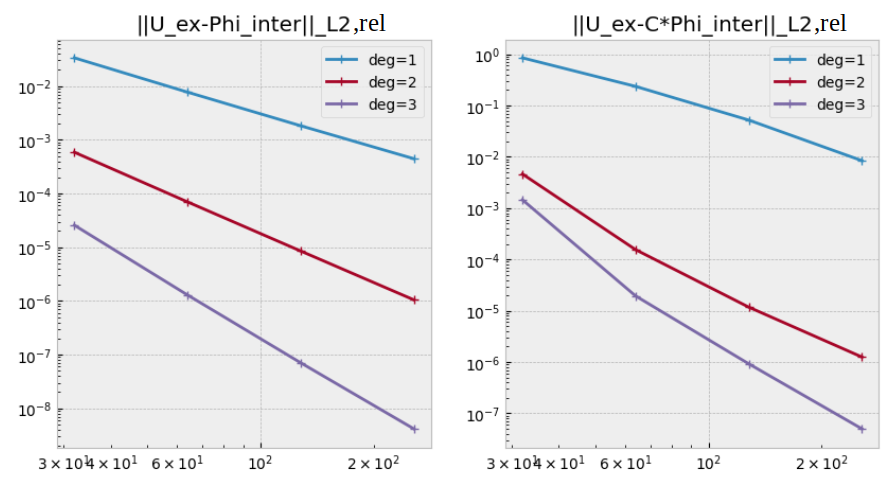
\includegraphics[width=0.6\linewidth]{cvg_sol_trigo.png}
\end{minipage}

On obtient
$$||u_{ex}-I_h u_{ex}||_{L^2(\Omega_h),rel}\sim h^{k+1}, \quad ||u_{ex}-CI_h u_{ex}||_{L^2(\Omega_h),rel}\sim h^{k+1}$$

\subsubsection*{f gaussienne}

On considère cette fois-ci $f$ gaussienne :
$$f(x,y) = \exp\left(-\frac{(x-\mu_0)^2 + (y-\mu_1)^2}{2\sigma^2}\right)\,, $$ 
avec $\sigma \sim \mathcal{U}([0.1,0.6])$ et $\mu_0, \mu_1 \sim \mathcal{U}([0.5-\sqrt{2}/4, 0.5+\sqrt{2}/4])$ à condition que $\phi(\mu_0, \mu_1) < -0.05$. \\

Dans un premier temps, on considère la solution de référence $u_{ex}$ comme étant une solution sur-raffinée obtenue par les EF standard (avec $h_{ex}\approx 0.006$ car $h_{ex}<<h_{FNO}$).  On interpole cette solution exacte (notre nouvelle level-set que l'on note $I_h u_{ex}$) dans $\mathbb{P}^k$ avec $k\in\{1,2,3\}$ et on fixe $C\in\mathbb{P}^1$.  


On obtient les résultats suivants :

\begin{minipage}{\linewidth}
	\centering
	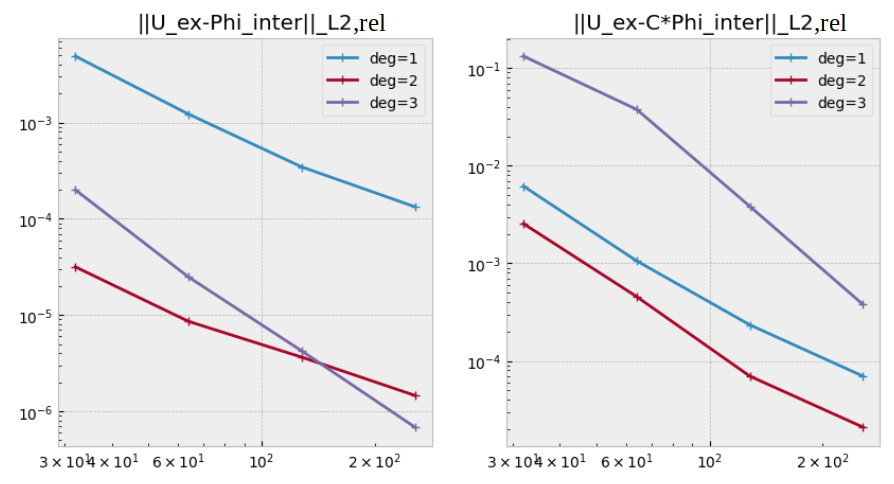
\includegraphics[width=0.6\linewidth]{cvg_f_gaussienne.png}
\end{minipage}

On obtient
$$||u_{ex}-I_h u_{ex}||_{L^2(\Omega_h),rel}\sim h^{k+1}, \quad ||u_{ex}-CI_h u_{ex}||_{L^2(\Omega_h),rel}\sim h^{k+1}$$

Cependant, il semblerait qu'il y ait un problème en $\mathbb{P}^3$ car l'erreur est plus grande qu'avec $k=1,2$. De plus la différence des erreurs en $×\mathbb{P}^1$ et en $\mathbb{P}^2$ est très petite. \\

Dans un second temps, on considère toujours la solution de référence $u_{ex}$ comme étant une solution sur-raffinée obtenue par les EF standard (avec $h\le 0.006$). On interpole cette fois-ci cette solution exacte (notre nouvelle level-set que l'on note $I_h u_{ex}$) dans $\mathbb{P}^{k+1}$ avec $k\in\{1,2,3\}$ et on prend $C\in\mathbb{P}^k$.  

On obtient les résultats suivants :

\begin{minipage}{\linewidth}
	\centering
	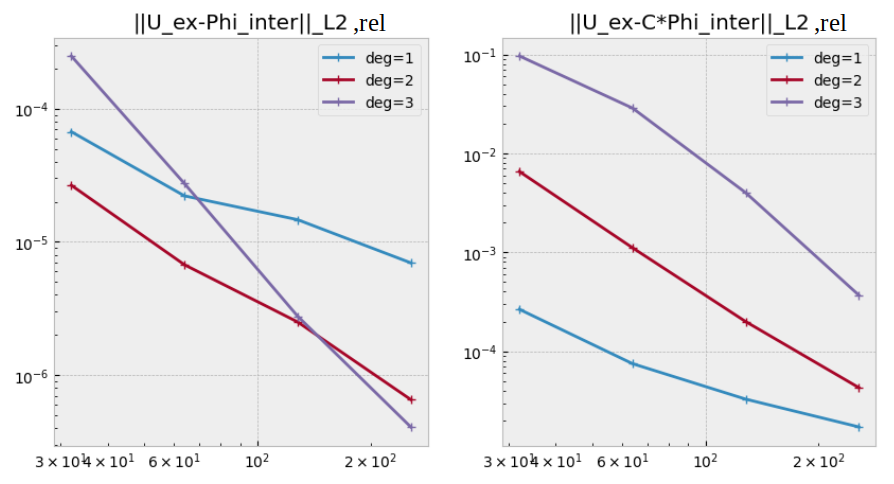
\includegraphics[width=0.6\linewidth]{cvg_f_gaussienne_2.png}
\end{minipage}

On obtient
$$||u_{ex}-I_h u_{ex}||_{L^2(\Omega_h),rel}\sim h^{k+1}, \quad ||u_{ex}-CI_h u_{ex}||_{L^2(\Omega_h),rel}\sim h^{k+1}$$

Cependant, il semblerait qu'il y ait un problème car l'erreur $\mathbb{P}^1$ est meilleure que l'erreur $\mathbb{P}^2$ qui elle-même est meilleure que l'erreur $\mathbb{P}^3$.


\subsection{Nouvelle idée FNO : Entraînement en $32\times 32 \; \mathbb{P}^2$}

On commence par générer $nb\_data$ données en $\mathbb{P}^2$ avec $nb\_vert=32$. Une première difficulté est de faire la conversion des résultats FEniCS en "image" Numpy. Ensuite, on entraîne le FNO avec ces données sur un certains nombres d'époques. On peut alors utiliser le FNO sur de nouvelles données (un échantillon test par exemple). On va ensuite corriger la sortie du FNO où une seconde difficulté est le passage de notre image Numpy (où chaque pixel représente la valeur de la solution en chacun des degré de liberté $\mathbb{P}^2$) à une Expression Fenics. Après la correction, on obtient la solution $\mathbb{P}^1$ (car $C\in\mathbb{P}^1$).

%\lstset{style=Python}

\textbf{Conversion FEniCS->Numpy : }

Cette conversion est effectuée lors de la génération des données. Le solveur PhiFEM nous fournit une expression FEniCS. Dans le cas $\mathbb{P}^1$, la fonction \textit{compute\_vertex\_values} de FEniCS nous permet de récupérer la valeur de la solution aux nœuds de notre maillage. En $\mathbb{P}^2$, c'est un peu plus compliqué, il faudra récupérer la valeur en chaque degré de liberté manuellement. Pour cela, on commence par récupérer les coordonnées de nos degrés de liberté en utilisant la fonction \textit{tabulate\_dof\_coordinates} de FEniCS. La complexité de cette méthode est que la numérotation FEniCS n'est pas la même que celle que l'on souhaiterais. C'est pour cela que l'on va devoir créer un mapping. Pour cela, on commence par récupérer le vecteur des coordonnées dont la première colonne contient $x$ et la deuxième contient $y$. On va rajouter une colonne contenant une nouvelle indexation de nos coordonnée. Puis, on trie cette matrice selon les ordonnées puis selon les abscisses. On obtient alors les coordonnées triées de bas en haut et de gauche à droite. La colonne contenant les indices est alors notre mapping. On peut alors ordonner l'expression et on obtient le tableau Numpy.

\textbf{Conversion Numpy->FEniCS : }

Cette conversion est utilisée pour convertir notre sortie de FNO en une fonction FEniCS pour la Correction. De la même manière, que pour la conversion dans le sens inverse, on crée un mapping qui nous permet d'associer chaque degré de liberté FEniCS aux valeurs Numpy.



\subsubsection{Solution analytique trigonométrique}

On considère encore la solution analytique trigonométrique suivante :
$$u_{ex}(x,y) = \frac{1}{\sin\left(k_1\frac{\pi}{2}\right)}\times\sin\left(k_1\frac{\pi}{2}\left(\frac{4}{\sqrt{2}}\right)^2\left((x-0.5)^2+(y-0.5)^2\right)\right)\times\cos\left(\frac{\pi}{2}\left(\frac{4}{\sqrt{2}}\right)^2\left((x-0.5)^2+(y-0.5)^2\right)\right)\,, $$ 

\newpage
Après entraînement sur 4000 époques voici les misfits obtenus : 

\begin{minipage}{\linewidth}
	\centering
	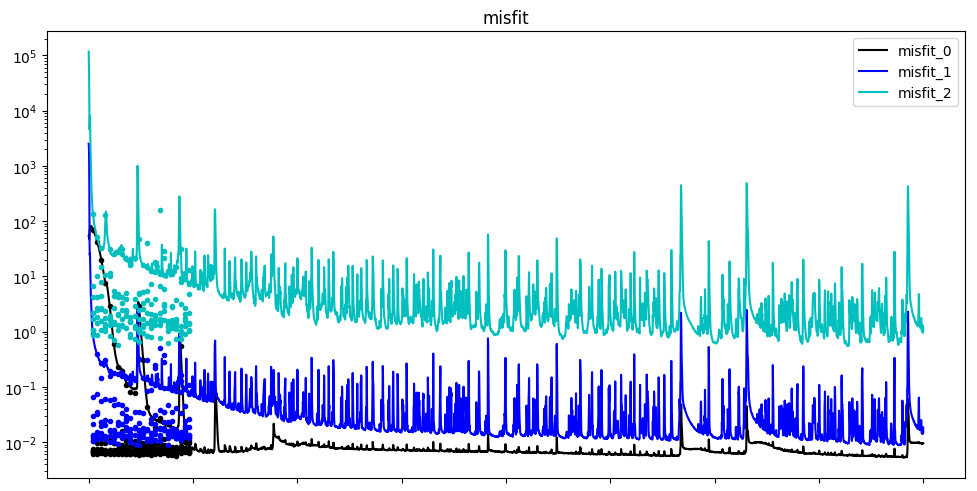
\includegraphics[width=0.7\linewidth]{FNO_trigo/misfits_sol_trigo.png}
\end{minipage}

\fbox{A RELANCER EN UNE TRAITE !}


\textbf{Échantillon de validation :}

On commence par calculer les erreurs en norme $L^2$ sur l'échantillon de validation. On considérera des "sous-modèle" qui seront sauvegarder toutes les 500 époques. A gauche, on a les erreurs sur l'échantillon de validations toutes les 1000 époques. A droite, il y a la moyenne, l'écart-type, le minimum et le maximum de l'erreur sur l'échantillon de validation pour chacun des sous-modèle (500,1000,1500,2000,2500,3000,3500 et 4000).

\begin{minipage}{0.48\linewidth}
	\centering
	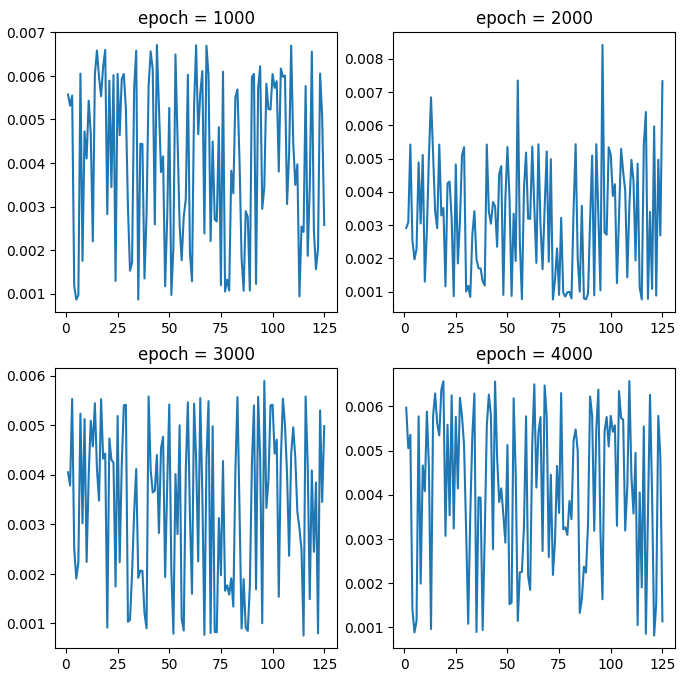
\includegraphics[width=0.8\linewidth]{FNO_trigo/erreur_val_sol_trigo.png}
\end{minipage}
\begin{minipage}{0.48\linewidth}
	\centering
	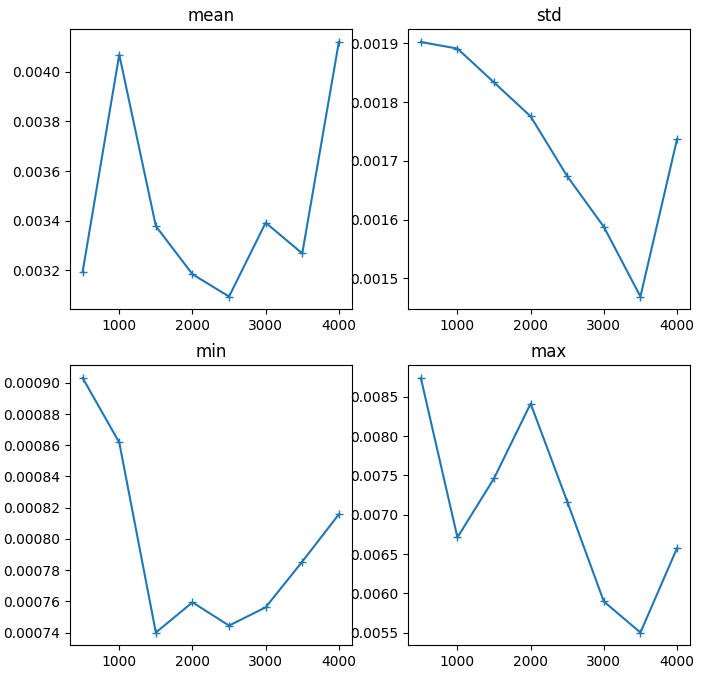
\includegraphics[width=0.8\linewidth]{FNO_trigo/infos_val_sol_trigo.png}
\end{minipage}

On réalise également un histogramme pour chacun des sous-modèles : 

\begin{minipage}{\linewidth}
	\centering
	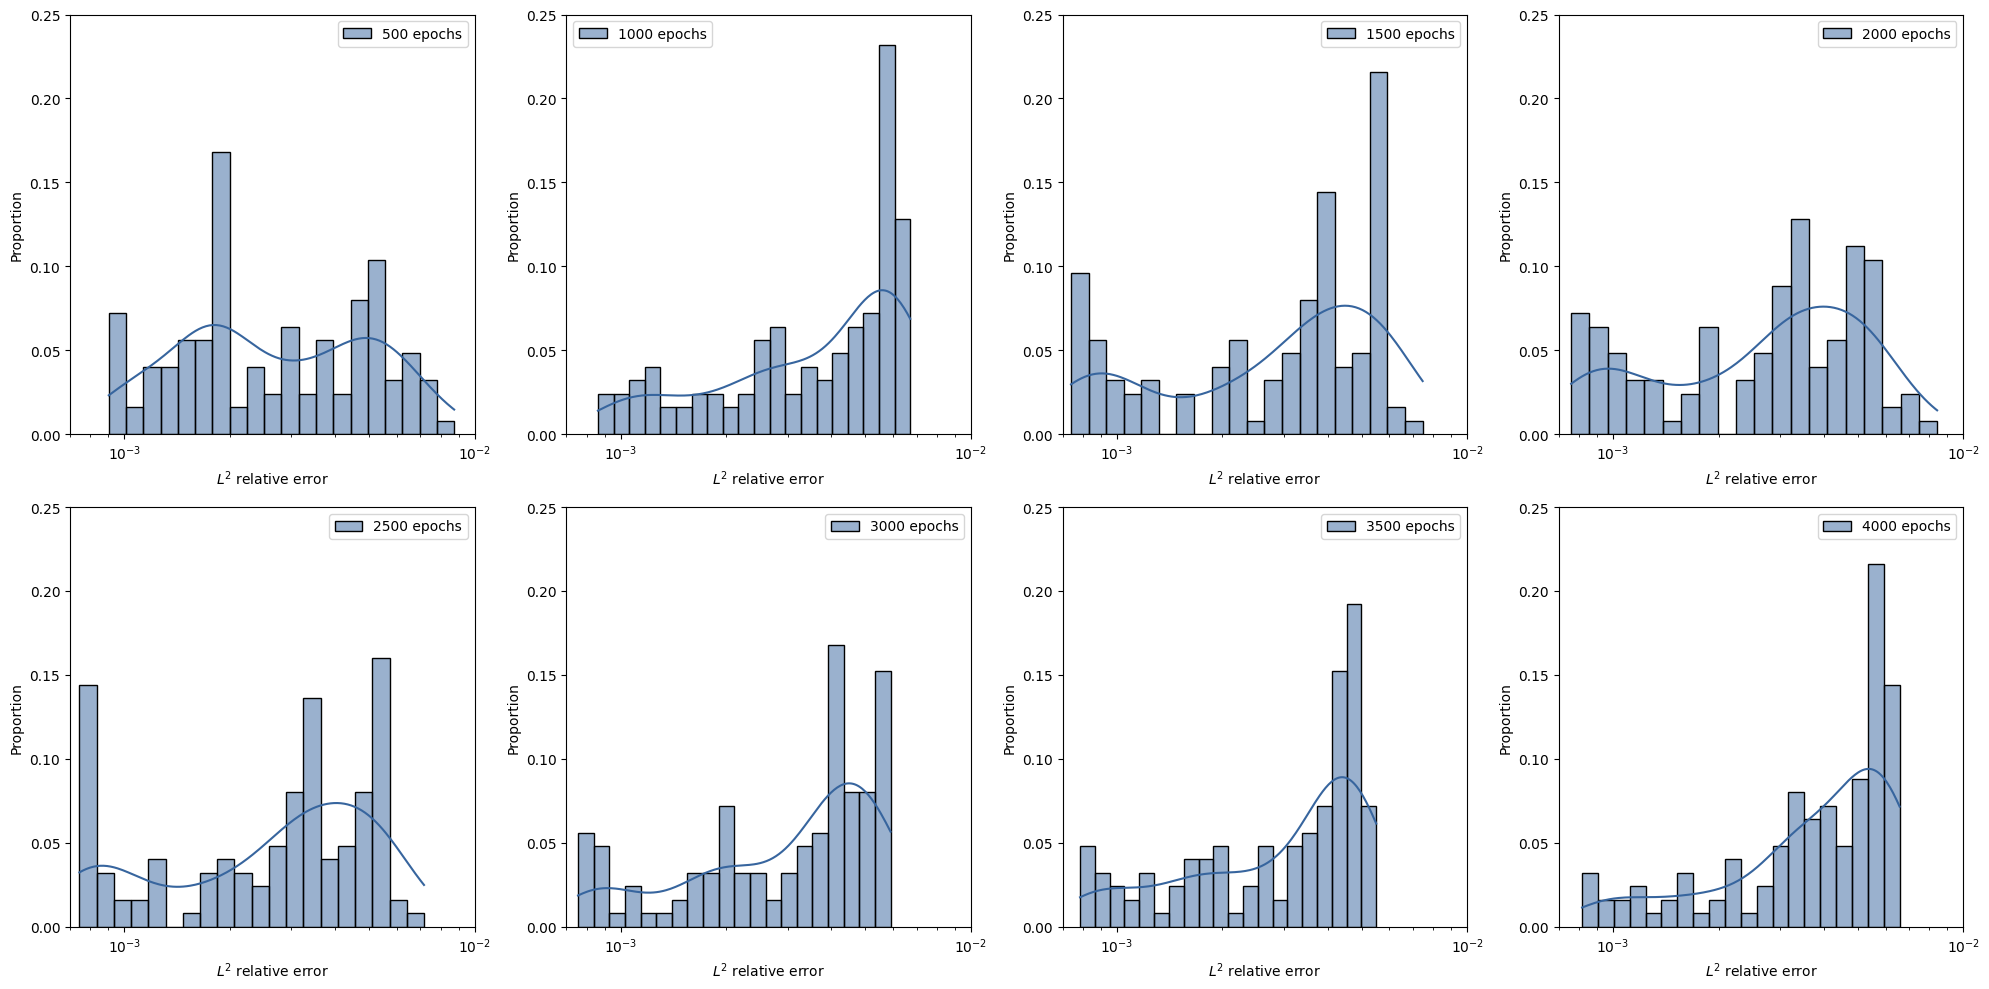
\includegraphics[width=0.8\linewidth]{FNO_trigo/histogram_val_sol_trigo.png}
\end{minipage}

\newpage

\textbf{Échantillon test :}
On s'intéresse exactement aux même résultats mais cette fois-ci sur un nouvel échantillon (un échantillon test de taille 100) :

\begin{minipage}{0.48\linewidth}
	\centering
	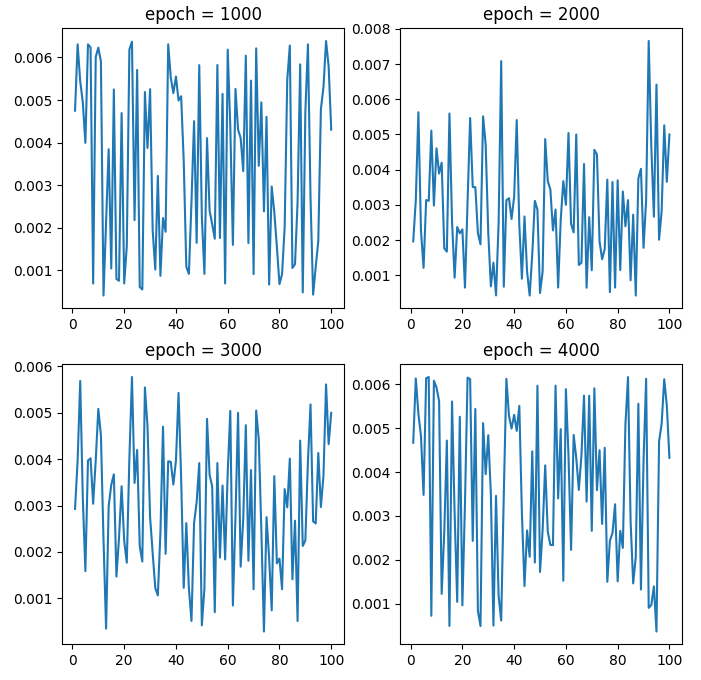
\includegraphics[width=0.8\linewidth]{FNO_trigo/erreur_test_sol_trigo.png}
\end{minipage}
\begin{minipage}{0.48\linewidth}
	\centering
	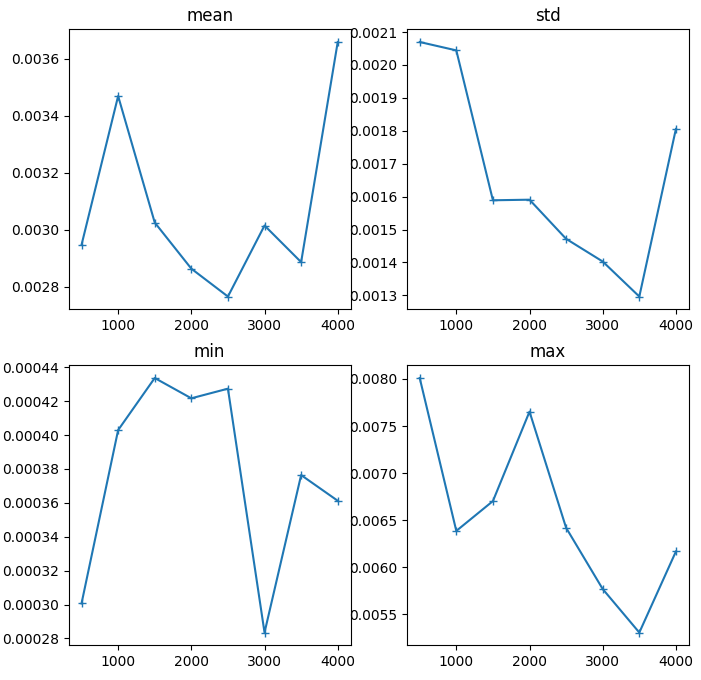
\includegraphics[width=0.8\linewidth]{FNO_trigo/infos_test_sol_trigo.png}
\end{minipage}

\begin{minipage}{\linewidth}
	\centering
	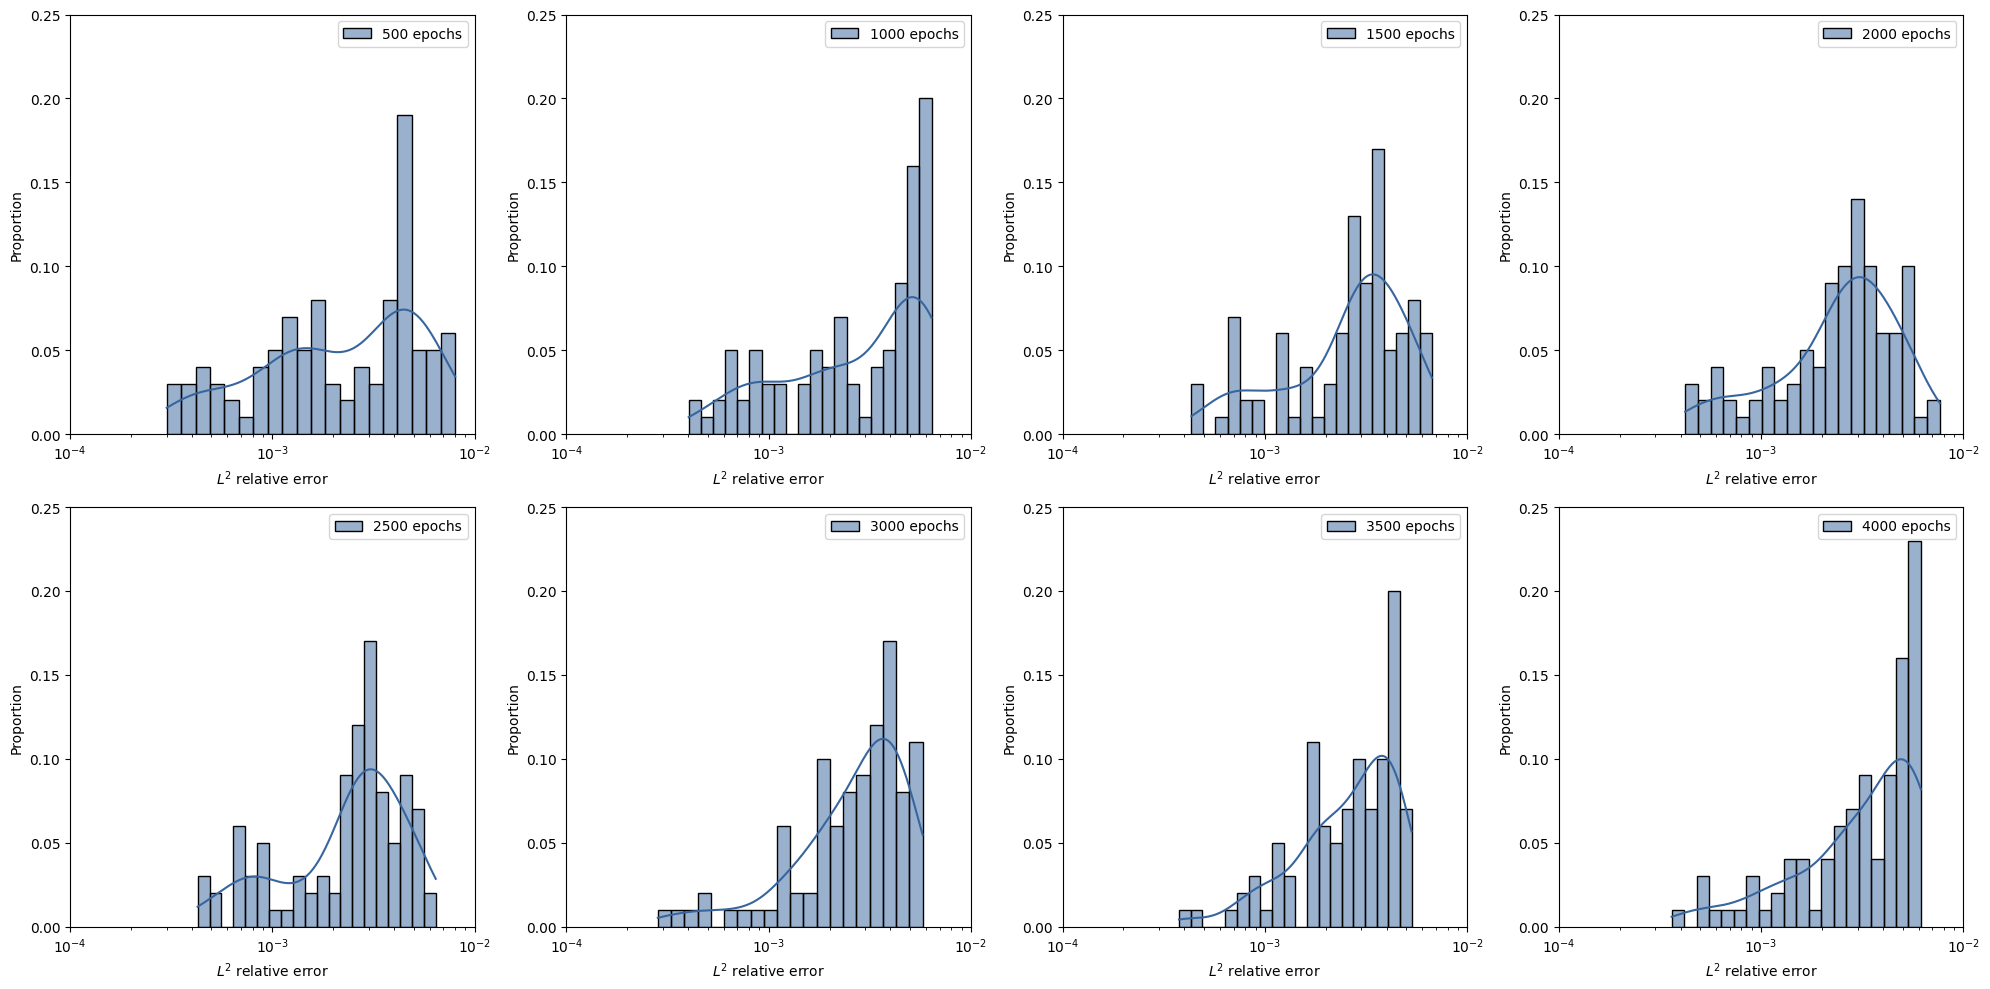
\includegraphics[width=0.8\linewidth]{FNO_trigo/histogram_test_sol_trigo.png}
\end{minipage}

\textbf{Résultat après correction : }

On cherche à tester la correction sur la sortie du FNO. Voici un exemple de résultat :

\begin{minipage}{\linewidth}
	\centering
	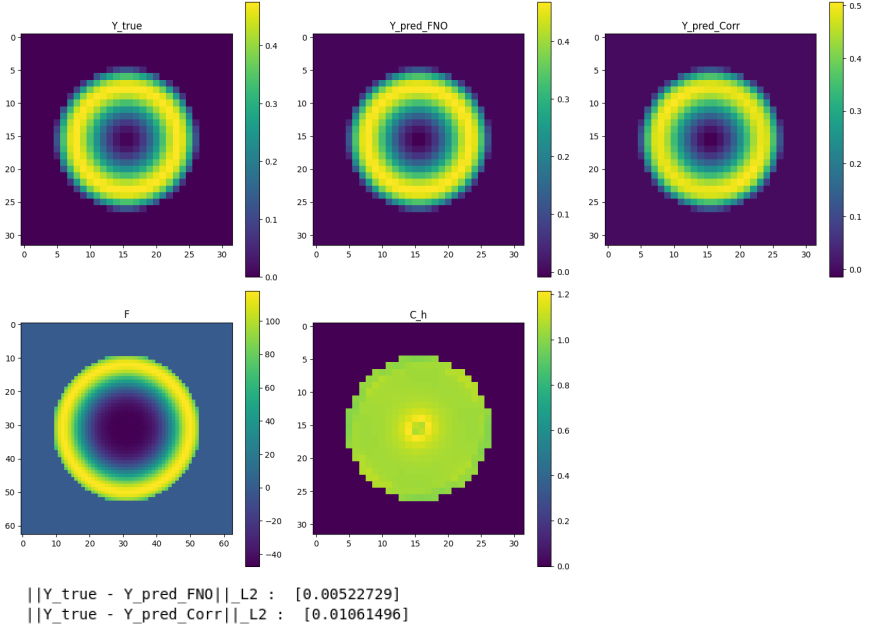
\includegraphics[width=0.68\linewidth]{FNO_trigo/resultat_sol_trigo.png}
\end{minipage}


On pense que les données précédentes ne varient pas assez et qu'elles sont donc trop facile à apprendre par le FNO. En effet, au bout de déjà 500 époques les erreurs semblent très bonnes. Ainsi la correction a du mal à être meilleure que la sortie du FNO. On va donc considérer un nouveau problème plus compliqué. On considère toujours le problème de poisson avec condition de Dirichlet homogène. On prend $f$ gaussienne et notre solution de référence sera une solution sur-raffinée obtenue par les éléments finis standard.

\subsubsection{f gaussienne}

On considère cette fois-ci $f$ gaussienne :
$$f(x,y) = \exp\left(-\frac{(x-\mu_0)^2 + (y-\mu_1)^2}{2\sigma^2}\right)\,, $$ 
avec $\sigma \sim \mathcal{U}([0.1,0.6])$ et $\mu_0, \mu_1 \sim \mathcal{U}([0.5-\sqrt{2}/4, 0.5+\sqrt{2}/4])$ à condition que $\phi(\mu_0, \mu_1) < -0.05$. \\

Après entraînement sur 4000 époques voici les misfits obtenus : 

\begin{minipage}{\linewidth}
	\centering
	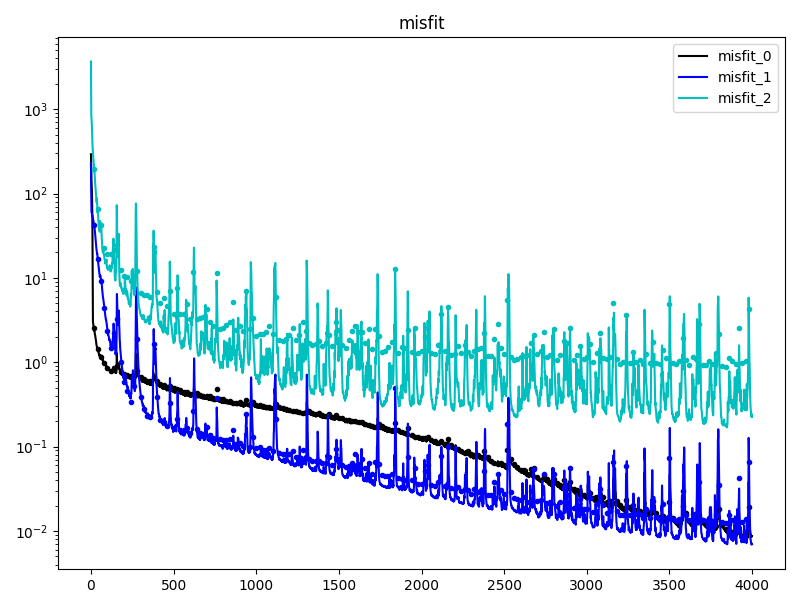
\includegraphics[width=0.6\linewidth]{FNO_gaussienne/misfits_f_gaussienne.png}
\end{minipage}

\textbf{Échantillon de validation :}

On commence par calculer les erreurs en norme $L^2$ sur l'échantillon de validation. On considérera des "sous-modèle" qui seront sauvegarder toutes les 500 époques. Voici les erreurs obtenus sur l'échantillon de validation pour chacun des sous-modèles :

\begin{minipage}{\linewidth}
	\centering
	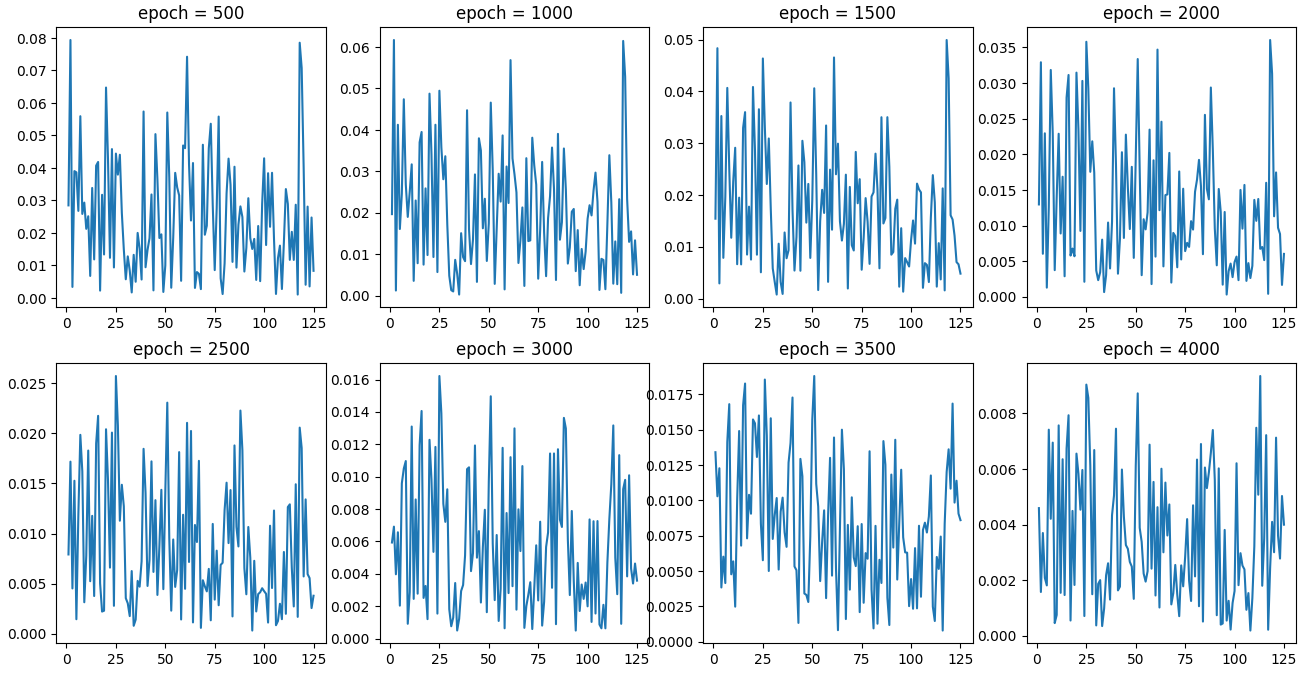
\includegraphics[width=0.9\linewidth]{FNO_gaussienne/erreur_val_f_gaussienne.png}
\end{minipage}

Voici la moyenne, l'écart-type, le minimum et le maximum de l'erreur sur l'échantillon de validation pour chacun des sous-modèle (500,1000,1500,2000,2500,3000,3500 et 4000) :

\begin{minipage}{\linewidth}
	\centering
	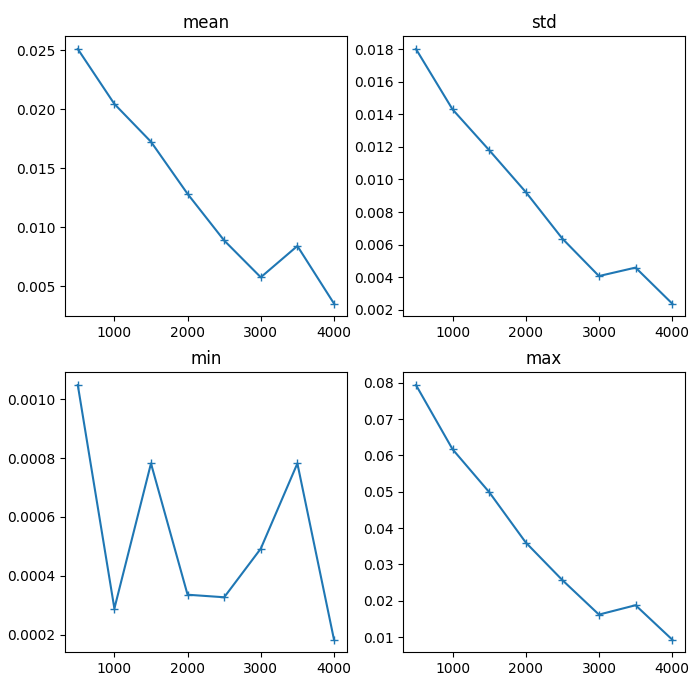
\includegraphics[width=0.4\linewidth]{FNO_gaussienne/infos_val_f_gaussienne.png}
\end{minipage}

On réalise également un histogramme pour chacun des sous-modèles : 

\begin{minipage}{\linewidth}
	\centering
	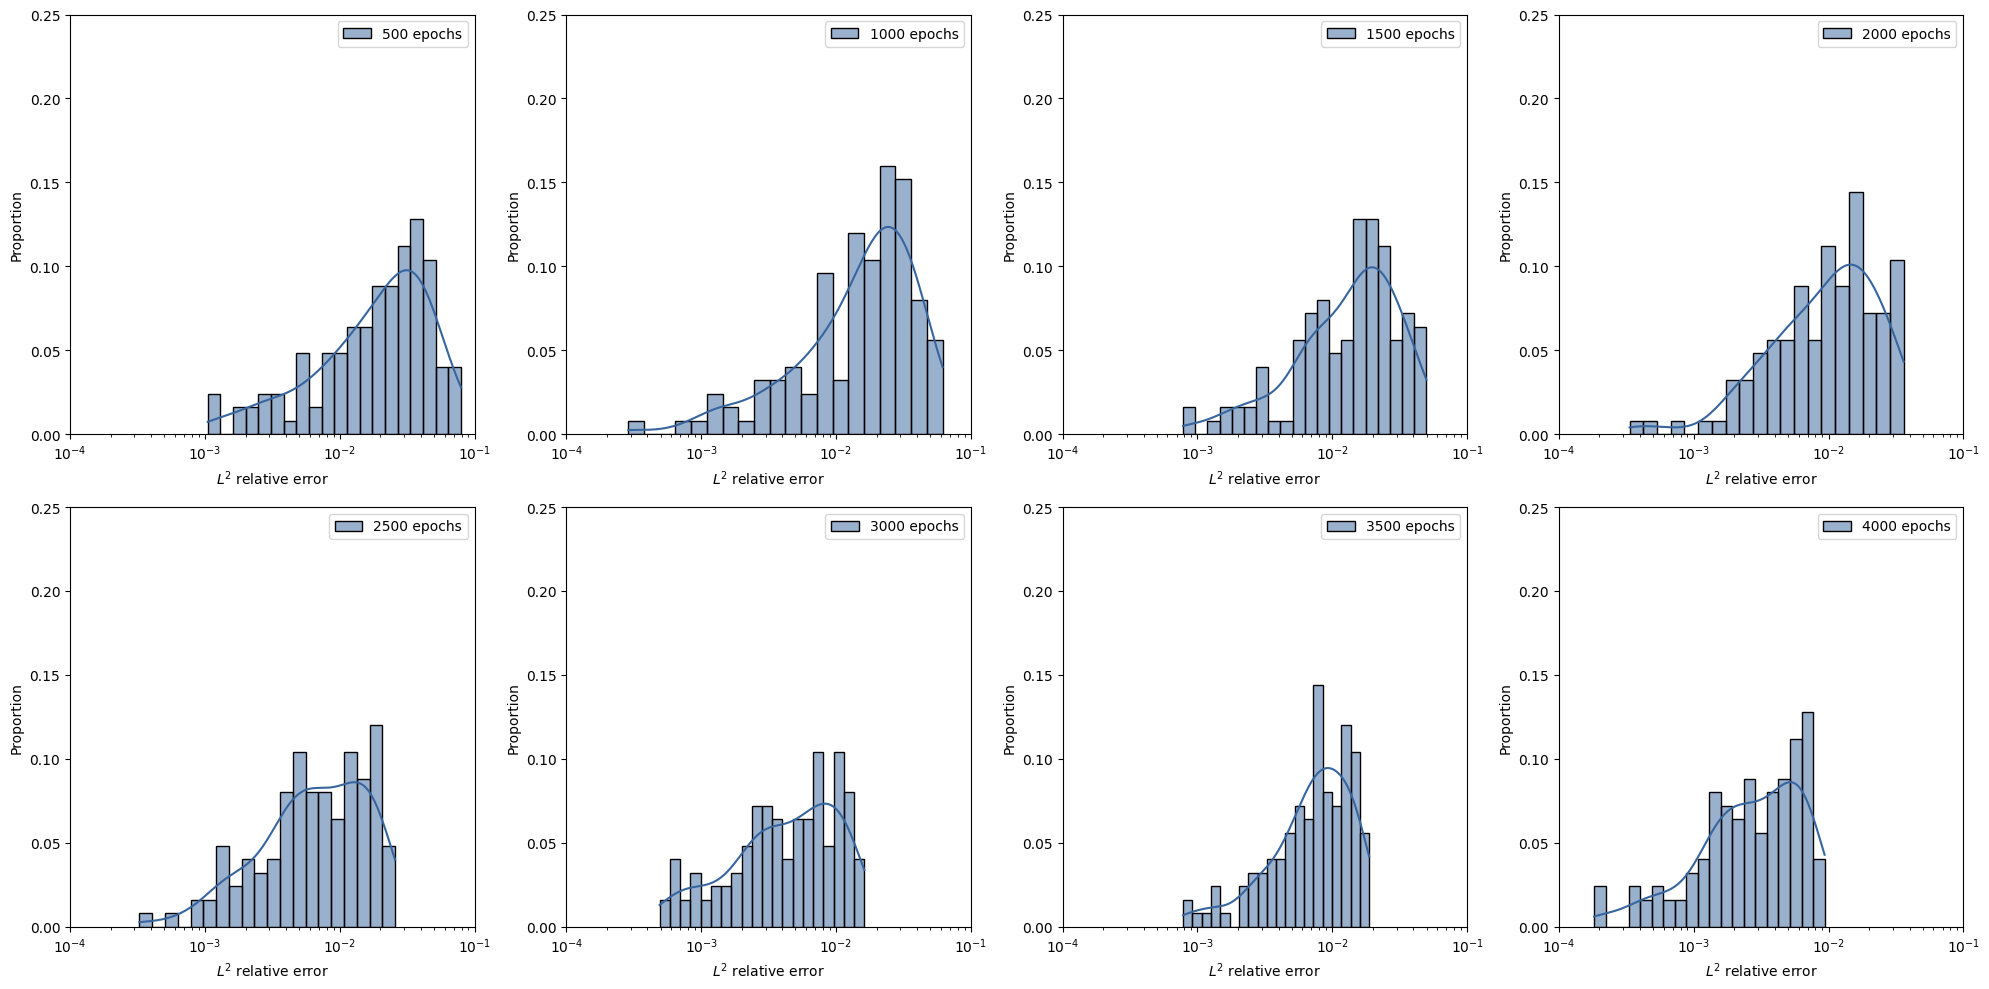
\includegraphics[width=0.8\linewidth]{FNO_gaussienne/histogram_val_f_gaussienne.png}
\end{minipage}

\textbf{Échantillon test :}
On s'intéresse exactement aux même résultats mais cette fois-ci sur un nouvel échantillon (un échantillon test de taille 100) :

\begin{minipage}{\linewidth}
	\centering
	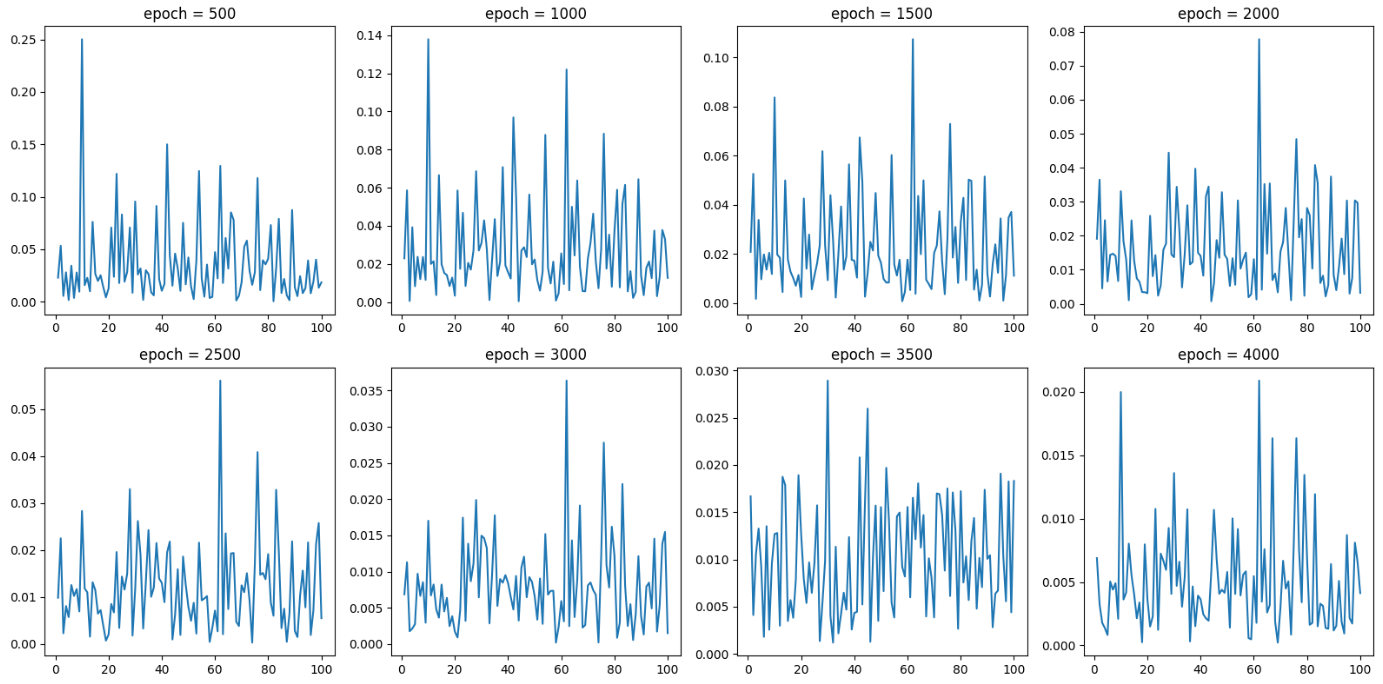
\includegraphics[width=0.9\linewidth]{FNO_gaussienne/erreur_test_f_gaussienne.png}
\end{minipage}

\begin{minipage}{\linewidth}
	\centering
	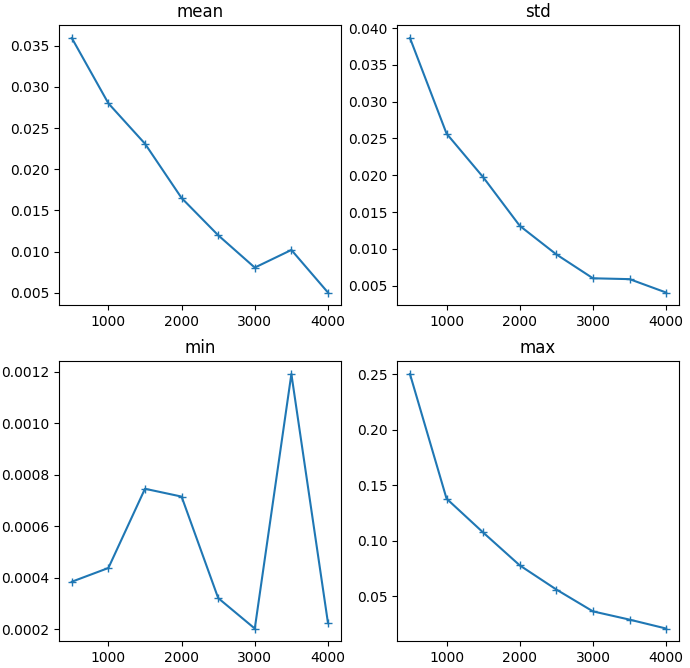
\includegraphics[width=0.45\linewidth]{FNO_gaussienne/infos_test_f_gaussienne.png}
\end{minipage}

\begin{minipage}{\linewidth}
	\centering
	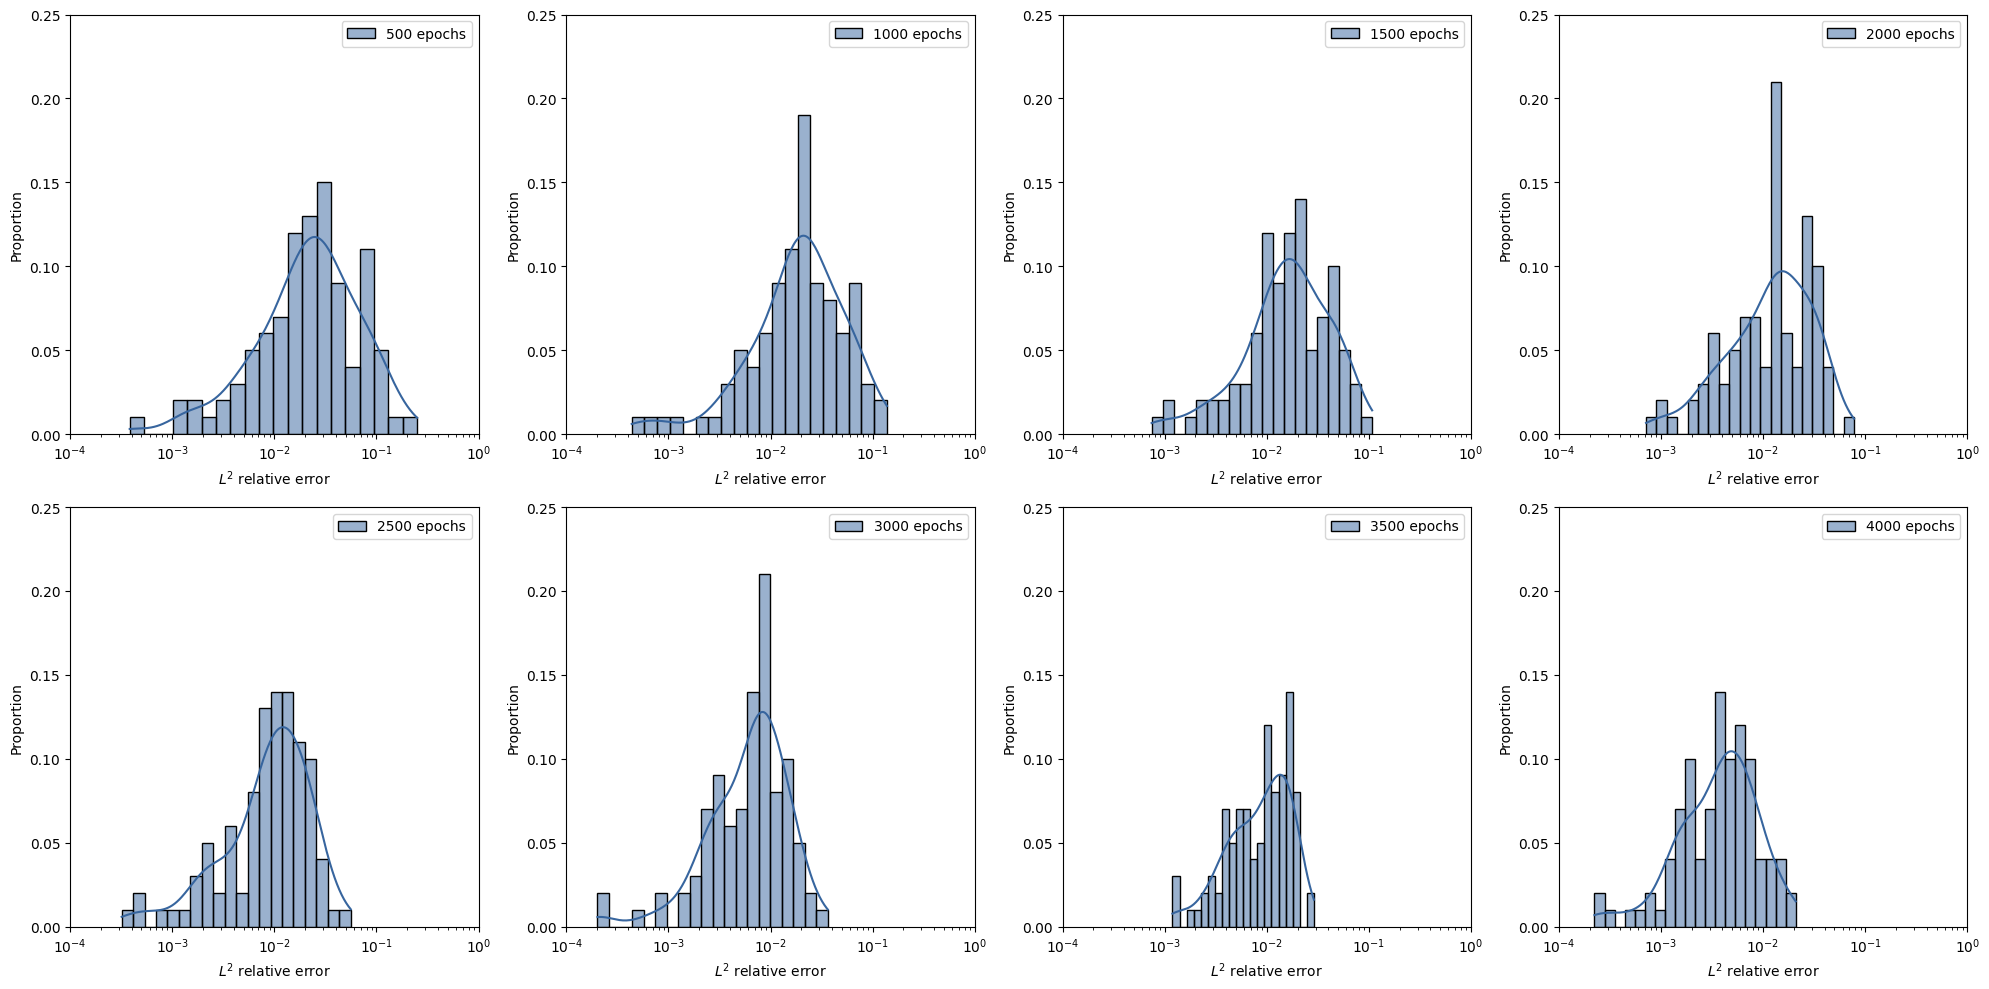
\includegraphics[width=0.8\linewidth]{FNO_gaussienne/histogram_test_f_gaussienne.png}
\end{minipage}

\textbf{Résultat après correction : }

On cherche à tester la correction sur la sortie du FNO. 

\begin{minipage}{\linewidth}
	\centering
	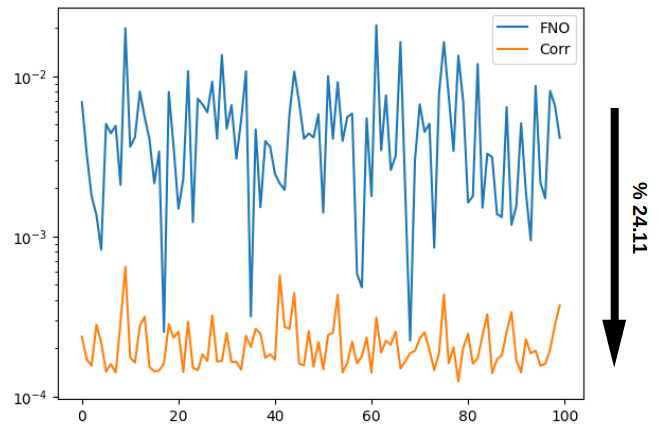
\includegraphics[width=0.68\linewidth]{FNO_gaussienne/resultats_test.png}
\end{minipage}